\documentclass[12pt,dvipdfmx,a4paper]{report}
\usepackage{comment}
\usepackage{./sty/eclepsf}
\usepackage{tascmac}
\usepackage{tabularx}
\usepackage{listliketab}
\usepackage[longnamesfirst,numbers]{natbib}
\usepackage[dvipdfmx]{graphics}
\usepackage[dvipdfmx]{graphicx}
\usepackage[dvipdfmx]{color}
\usepackage{subfigure}
\usepackage{alltt}
\usepackage{here}
\usepackage{afterpage}
\usepackage{graphicx}
\usepackage{here}
\usepackage{amsmath, amssymb}
\usepackage{type1cm}
\usepackage{yquant}
\usepackage{tikz}
\usetikzlibrary{quantikz}
\usepackage{./sty/ncodeline}
%\usepackage[dvipdfmx, colorlinks, breaklinks,%
\usepackage[dvipdfmx, breaklinks,bookmarks=true, bookmarksnumbered=true,bookmarkstype=toc, bookmarksopen=true,bookmarksopenlevel=3,pdftitle={RG}]{hyperref}
\usepackage{bookmark}
\usepackage{mathtools}
\usepackage{tikz}
\usetikzlibrary{automata, positioning, arrows}
\usepackage[T1]{fontenc}
\usepackage{algorithm}
\usepackage{algpseudocode}
\usepackage{array}
\usepackage{amsthm}

\AtBeginDvi{\special{pdf:tounicode EUC-UCS2}}

\usepackage{fancyhdr}

\usepackage{./sty/doxygenorig}

\usepackage{indentfirst}
\usepackage{url}
\usepackage{listings,./sty/jlisting}
\usepackage{float}
\usepackage{tabularx}
\usepackage{setspace}
\graphicspath{ {./images/} }
\newtheorem{theorem}{Theorem}

\def\lstlistingname{プログラム}

\lstset{%
 language={C++},
 %backgroundcolor={\color[gray]{.85}},%
 basicstyle={\small\ttfamily},%
 identifierstyle={\small},%
 commentstyle={\small\itshape},%
 keywordstyle={\small\bfseries},%
 ndkeywordstyle={\small\ttfamily},%
 stringstyle={\small\ttfamily},
 frame={tb},
 framesep=1zw,
 breaklines=true,
 numbers=left,%
 xrightmargin=0zw,%
 xleftmargin=1.5zw,%
 numberstyle={\scriptsize},%
 stepnumber=1,
 numbersep=1zw,%
 lineskip=-0.5ex%
}

\usepackage{amssymb}
%\usepackage{supertabular,multirow}

\usepackage{array}
\newcolumntype{M}[1]{>{\centering\arraybackslash}m{#1}}

% A4  size: 297mm*210mm %1pt = 0.35mm
\setlength{\topmargin}{-3.4mm} % 10pt 25.4mm - 3.4mm = 22mm
\setlength{\oddsidemargin}{-0.4mm} % 25.4mm - 0.4mm = 25mm
\setlength{\evensidemargin}{-0.4mm} % 25.4mm - 0.4mm = 25mm
\setlength{\textheight}{231mm} % 660pt % original is 225.75mm 645pt
\setlength{\textwidth}{160mm} % 457pt

\renewcommand{\topfraction}{.99}
\renewcommand{\textfraction}{.0}
\renewcommand{\floatpagefraction}{.99}
\renewcommand{\bibname}{Reference}
\DeclareMathOperator{\tr}{tr}

\pagestyle{fancy}
\lhead[]{}

% タイトル
\def\title{Link Management in a Quantum Network}
% 英語タイトル
\def\etitle{Link Management in a Quantum Network}
% 著者(日本語)
\def\author{Makoto Nakai}
% 著者(英語)
\def\eauthor{Makoto Nakai}
% 学部・研究科
\def\dept{Keio University Graduate School of Media and Governance}
% 学部・研究科(英語)
\def\edept{Keio University Graduate School of Media and Governance}

\begin{document}

\pagenumbering{roman}
\begin{titlepage}
  \begin{spacing}{1.6}
  \begin{center}
  \Large 
   \textbf{Master's Thesis (Academic Year 2023)}\\
   \hspace*{\fill}\\
   \hspace*{\fill}\\
   \hspace*{\fill}\\
   \LARGE 
   \textbf{Link Management in a Quantum Network}
   \vspace{8.5cm}
   \end{center}
   \begin{flushleft}
       \Large 
       \textbf{Keio University \\ Graduate School of Media and Governance}
   \end{flushleft}
   \begin{flushright}
    \Large  
    \textbf{Makoto Nakai} 
   \end{flushright}
  \end{spacing}
\end{titlepage}

\thispagestyle{empty}

Abstract of Master's Thesis - Academic Year 2023
\begin{center}
\begin{large}
\begin{tabular}{|p{0.97\linewidth}|}
    \hline
      \etitle \\
    \hline
\end{tabular}
\end{large}
\end{center}

~ \\
Quantum networking is a new networking paradigm that allows specialized network nodes to share quantum states in order to achieve new applications.  RuleSet-based communication protocol is known to be one of the practical communication protocols to establish a scalable quantum network.
 Ideally, the network should be able to handle the multiple connections and the subsequence management of the link-level Bell pairs in order to improve the overall performance and the aggregate use of the available resource on the network, even when the number of the active connections changes. 
 However, the current state of the protocol only allows the establishment of a single connection and lacks the ability to terminate it and release the allocated resources on the link level.
 This thesis proposes the link management protocol for quantum network that allows the allocation and release of Bell pairs on the link level, which is the key to change of the number of active connections.
 It discusses the relationship between the connection management and the resource management in the link level. The behavior of the proposed protocol is validated by a set of numerical simulations on an existing quantum networking simulator.
~ \\
Keywords : \\
\underline{1. Quantum Networking},
\underline{2. RuleSet-Based Communication Protocol},
\underline{3. Networking Protocol},
\begin{flushright}
\edept \\
\eauthor
\end{flushright}

\thispagestyle{plain}
\clearpage

\tableofcontents\thispagestyle{plain} %目次
\clearpage
\listoffigures\thispagestyle{plain} %図目次
\clearpage
\listoftables\thispagestyle{plain} %表目次
\clearpage

\pagenumbering{arabic}
\chapter{Introduction}
\label{introduction}

\section{Background}
\label{introduction:background} 

The recent development of quantum technologies such as quantum computing, quantum networking and quantum sensing are expected to provide new capabilities. 
For example, quantum processors can theoretically simulate quantum systems whose size are intractable even for their classical equivalence.
The key to realize these new applications is quantum effect, such as superposition and entanglement, both of which cannot be observed in the classical world.

However, there are two major problems for transmitting quantum data to a distance location, which is required in certain situations such as distributed quantum computing.
One is "non-cloning theorem", which is the fact that quantum state cannot be copied. Unlike classical network, it is almost impossible to neither amplify a quantum state or send it forward because the quantum state will be heavily corrupted by the high probability of loss and high error rate.
The other problem is that it is so difficult to establish a bell pair between nodes separated by a long distance, again due to a photon will be spoiled by the physical noise and photon loss.

These two problems can be solved by using particular type of nodes called quantum repeaters. Quantum repeaters perform entanglement swapping and purification, each of which extends two neighboring bell pairs to a single longer bell pair, and improves the fidelity of the bell pair, respectively.
These operations end up with generating an end-to-end bell pair that can be used by quantum teleportation, which is the protocol to send an arbitrary quantum state to a distant location. 

Entanglement swapping and purification involve requires frequent message exchange with neighboring nodes in order to coordinate actions, such as entanglement swapping and purification, with neighboring nodes and those communication slow down the generation of an end-to-end bell pair.
However, a communication protocol called RuleSet-based communication protocol solves this problem by distribute an object called RuleSet, which a sequence of operations execute to each node. This feature reduces the amount of unnecessary communication and improves the scalability of the entire network.

\section{Research Contribution}
\label{introduction:research-contribution}

Multiple connections should be established simultaneously in order to enhance the overall performance and robustness of the entire network and the same thing can be applied to quantum network. 
However, the previous work only proposes the method to allocate required physical bell pairs and establish a single end-to-end bell pair, in other word, an single connection by consuming those physical resources.
This thesis proposes a protocol to realize three important tasks, which are the negotiation about what set of connections are going to be established, the one about when to switch from those in the previous round, and coordinated resource management between two nodes connected by each link.
It also discusses the updated procedure of establishing a new connection and tearing down one of the existing connections while several connections are being established by applying the proposed protocol.
The approach presented in this thesis is validated by the simulation of RuleSet-based quantum networks under several circumstances.

\section{Thesis Structure}
\label{introduction:thesis-structure} 
% 本論文における以降の構成は次の通りである.

The structure of this thesis is as follows. 

Chapter \ref{background} provides the background knowledge to understand the key concepts readers would encounter throughout this thesis.

Chapter \ref{related works} explains the detail of RuleSet-based quantum networking.

Chapter \ref{problem-definition} presents the problem that this thesis addresses.

Chapter \ref{proposal} offers the overview of the link management protocol and the messages required for its negotiation process.

Chapter \ref{simulation} provides how link management protocol proposed in this thesis will be triggered after the process of connection setup and teardown. It also includes the pseudocode of methods that the node software need to execute and messages outside of the link management protocol.

Chapter \ref{evaluation} presents several scenarios used to validate this protocol.

Chapter \ref{conclusion} offers the conclusion of this thesis and discusses future works.

% ~\ref{background}章では,背景を述べる.
% ~\ref{issue}章では,本研究における問題の定義と,解決するための要件の整理を行う.
% ~\ref{proposed}章では,本研究の提案手法を述べる.
% ~\ref{implementation}章では,~\ref{proposed}章で述べたシステムの実装について述べる.
% ~\ref{evaluation}章では,\ref{issue}章で求められた課題に対しての評価を行い,考察する.
% ~\ref{conclusion}章では,本研究のまとめと今後の課題についてまとめる.


%%% Local Variables:
%%% mode: japanese-latex
%%% TeX-master: "../thesis"
%%% End:

\chapter{Background}
\label{background}

\section{Quantum Physics}

This subsection provide the fundamental knowledge of quantum physics, which will make readers feel familiar with the concept and notations that they will encounter throughout this thesis.

%TODO: List four postulate of quantum physics 

\subsection{Pure State}

Pure state is the representation of quantum state of the whole system without the assumption of external noise.

\subsubsection{Quantum Bit}

A conventional computer uses a bit to represent a basic unit of information, which are 0 and 1. A basic unit of quantum information, on the other hand is called a quantum bit (or \textbf{qubit} in short) are $|0\rangle$ and $|1\rangle$, each of which can be described in the form of a vector. 

For example  
 $$|0\rangle = \Big[
\begin{array}{c}
1 \\
0 \\
\end{array}
\Big]
$$

$$|1\rangle = \Big[
\begin{array}{c}
0 \\
1 \\
\end{array}
\Big]$$

The state of a single qubit $|\psi\rangle$ can be described as follows.
$$ |\psi\rangle = \alpha |0\rangle + \beta |1\rangle \,(\alpha, \beta \in \mathbb{C}, |\alpha|^2+|\beta|^2=1)$$.
 After the operation called measurement, the quantum state would be collapsed into either 0 or 1.  The measurement probability of 0 is $|\alpha|^2$ and that of 1 is $|\beta|^2$. In other words, a single qubit can take both states probabilistically at the same time.  
 
 For instance, a qubit can be 
 
 \begin{equation}
	|\psi\rangle = \frac{1}{\sqrt{2}}|0\rangle + \frac{1}{\sqrt{2}}|1\rangle \tag{1}
\end{equation}

 whose measurement probability of 0 and 1 is 50\% and 50\% respectively.

\subsubsection{Bloch Sphere}
Because $|\alpha|^2 + |\beta|^2 = 1$, the notation of a single qubit state can be represented like this.

\begin{equation}
|\psi\rangle = e^{i\gamma} (\cos{\frac{\theta}{2}} + e^{i\phi} \sin{\frac{\theta}{2}}) (\gamma, \phi, \theta \in \mathbb{R})
\end{equation}.

Because $e^{i\gamma}$ is just a global state, it can be ignored and the same state can be rewritten like this.

\begin{equation}
 |\psi\rangle =  \cos{\frac{\theta}{2}} + e^{i\phi} \sin{\frac{\theta}{2}} (\phi, \theta \in \mathbb{C})
\end{equation}

Because the equation above has two parameters,  any pure single qubit state can be considered as a point on the surface and its geometric representation is called \textbf{Bloch sphere}.

\begin{figure}[ht]
  \centering
  \tikz{
    \tikzstyle{st}=[lightgray, fill, fill opacity=0.2];
    \coordinate(o)at(0,0); 
    \draw(o)circle(2cm); 
    \draw[fill](o)circle(1.5pt);%origin
    \draw[st](o)--(56.7:0.4)arc(56.7:90.:0.4)--cycle;%theta angle
    \draw(0.18,0.6)node{$\theta$};
    \draw[st](o)--(-135.7:0.4)arc(-135.7:-33.2:0.4)--cycle;%varphi angle
    \draw(0.14,-0.58)node{$\varphi$};
    \draw[->](o)--(-0.81,-0.79) node[above left]{\ $x$};%x
    \draw[->](o)--(2,0)node[right]{$y$};%y
    \draw[->](o)--(0,2)node[below right]{$z$}node[above]{\ $\ket{0}$};%z |0>
    \draw[rotate around={0.:(0.,0.)},dashed](0,0)ellipse(2cm and 0.9cm);%ellipse
    \draw[thick,->](o)--(0.70,1.07)node[above]{\ $\ket{\psi}$};%state vector
    \draw[densely dotted,->](o)--(0,-2)node[below]{\ $\ket{1}$};%-z |1>
    \draw[dotted](o)--(0.7,-0.46)--(0.7,1);%triangle
  }
    
\newpage
\caption{Bloch Sphere}
\end{figure}

\subsubsection{Multi-Qubit State}
  The quantum state for multi-qubits is a \textbf{tensor product} of a state vector of each qubit.  The general notation of two qubit state is
  
\begin{flalign}
    |\psi\rangle & = (\alpha |0\rangle + \beta |1\rangle) \otimes  (\gamma |0\rangle + \delta |1\rangle) \\
    & = \alpha \gamma |00\rangle + \alpha \delta |01\rangle + \beta \gamma |10\rangle + \beta \delta |11\rangle \\ 
   & (\alpha, \beta, \gamma, \delta \in \mathbb{C}, |\alpha|^2+|\beta|^2+|\gamma|^2+|\delta|^2=1)
 \end{flalign}.
  
  For example, the state $|00\rangle$ is equal to 
  
\begin{equation}
  \Big[
\begin{array}{c}
1 \\
0 \\
\end{array}
\Big]
\otimes
 \Big[
\begin{array}{c}
1 \\
0 \\
\end{array}
\Big]
= \Bigg[
\begin{array}{c}
1 \\
0 \\
0 \\
0 \\
\end{array}
\Bigg]
\end{equation}.

 However, some quantum states such as
 
 \begin{equation}
 	|\psi\rangle = \frac{1}{\sqrt{2}}|00\rangle + \frac{1}{\sqrt{2}}|11\rangle
 \end{equation}
 
 cannot be decomposed into quantum state of each qubit.  These special quantum states are called \textbf{entangled} states.

 \subsection{Mixed State}
 %TODO: Add general principles of density metrics and their proofs
%TODO: ADD proof that a density matrix is positive semidefinite

 Mixed state is another representation of quantum state in more general cases, such as the presense of physical error.
Mixed state is described in the form of a matrix which is called density matrix.  Assume quantum system takes one of their collections $\{|\psi_i\rangle\}$ ($i$ is an index) with the probability of $p_i$.

\subsubsection{Mixed State}

The density matrix of this system $\rho$ is described by 

\begin{equation}
  \rho = \sum_i p_i |\psi_i\rangle\langle\psi_i|
\end{equation}

\subsubsection{Evolution}

The quantum system after applying a unitary operator $U$ is the following.
\begin{equation}
  \rho = \sum_i p_i |\psi_i\rangle\langle\psi_i| \xrightarrow{U} \sum_i p_i U|\psi_i\rangle\langle\psi_i|U^{\dagger}
\end{equation}

\subsubsection{Measurement}

Suppose one performs measurement on a quantum state $|\psi_i\rangle$ using a measurement operator $M_m$. 

Then, the measurement probability of $m$ is 
\begin{equation}
  p(m|i) = \langle\psi_i|M^{\dagger}_m M_m|\psi_i\rangle = tr(M^{\dagger}_m M_m|\psi_i\rangle\langle\psi_i|)
\end{equation}

The measurement probability of $m$ from the collection of state $\{|\psi_i\rangle\}$ is 
\begin{equation}
  \begin{split}
    p(m) &= \sum_i p_i p(m|i) \\ 
    &= \sum_i p_i \langle\psi_i|M^{\dagger}_m M_m|\psi_i\rangle \\
    &= \sum_i p_i \tr(M^{\dagger}_m M_m|\psi_i\rangle\langle\psi_i|) \\
    &= \tr(M^{\dagger}_m M_m \rho)
  \end{split}
\end{equation}

The quantum state after the measuring $|\psi_i\rangle$ is 
\begin{equation}
  |\psi^m_i\rangle = \frac{M_m|\psi^m_i\rangle}{\sqrt{\langle \psi^m_i|M^{\dagger}_m M_m|\psi^m_i\rangle}}
\end{equation}

The corresponding density matrix is
\begin{equation}
  \begin{split}
    \rho_m = \sum_i p(i|m)|\psi^m_i\rangle\langle\psi^m_i| = \sum_i p(i|m)\frac{M_m|\psi_i\rangle\langle\psi_i|M^{\dagger}_m}{\sqrt{\langle \psi^m_i|M^{\dagger}_m M_m|\psi^m_i\rangle}}
  \end{split}
\end{equation}

\begin{equation}
  \begin{split}
    p(i|m) &= \frac{p(m, i)}{p(m)} = \frac{p(m|i)p_i}{p(m)} \\
    &= \frac{\tr(M^{\dagger}_m M_m \rho) p_i}{\tr(M^{\dagger}_m M_m \rho)} \\
    &= p_i
  \end{split}
\end{equation}

Therefore, the state can also be described by the equation
\begin{equation}
  \begin{split}
    \rho_m &= \sum_i p_i \frac{M_m|\psi_i\rangle\langle\psi_i|M^{\dagger}_m}{\tr(M^{\dagger}_m M_m \rho)} \\
    &= \frac{M_m \rho M^{\dagger}_m}{\tr(M^{\dagger}_m M_m \rho)}
  \end{split}
\end{equation}



 \subsection{Fidelity}
  %TODO: Add proof that the square root of density matrix exists in the appendix
  %TODO: Mention the fact above in this subsection.

 Fidelity is one of the distance between two quantum state. the fidelity of quantum state $\rho$ and $\sigma$ is
 \begin{equation}
  \begin{split}
    F(\rho, \sigma) &= \tr{\sqrt{\rho^{\frac{1}{2}}\sigma\rho^{\frac{1}{2}}}} \\
  \end{split}
\end{equation}

For instance, if they commute and diagonal in the same basis like the following,
 \begin{equation}
  \begin{split}
    \rho &= \sum_i r_i |i\rangle\langle i|, \sigma= \sum_i s_i |i\rangle\langle i|\\
  \end{split}
\end{equation}

The fidelity between these two states would be
\begin{equation}
  \begin{split}
    F(\rho, \sigma) &= \tr{\sqrt{\sum_i r_i s_i |i\rangle\langle i|}} \\
    &= \tr(\sum_i \sqrt{r_i s_i} |i\rangle\langle i|) \\
    &= \sum_i \sqrt{r_i s_i}
  \end{split}
\end{equation}

The fidelity between a pure state $|\psi\rangle$ and a mixed state $\rho$ is 
\begin{equation}
  \begin{split}
    F(\psi, \rho) &= \tr{\sqrt{\langle\psi|\rho|\psi\rangle|\psi\rangle\langle\psi|}} \\
    &= \sqrt{\langle\psi|\rho|\psi\rangle}
  \end{split}
\end{equation}

\section{Quantum Operations}
\subsection{I Gate}

I gate is equal to the 2 $\times$ 2 identity matrix, which is 

\begin{equation}
I = \begin{bmatrix}
1 & 0 \\
0 & 1 \\
\end{bmatrix}
\end{equation}.

For example,

\begin{equation}
 I|0\rangle = \begin{bmatrix}
1 & 0 \\
0 & 1 \\
\end{bmatrix} 
\left[
\begin{array}{c}
1 \\
0 \\
\end{array}
\right]
= \left[
\begin{array}{c}
1 \\
0 \\
\end{array}
\right]
= |0\rangle
\end{equation}

\begin{equation}
I|1\rangle = \begin{bmatrix}
1 & 0 \\
0 & 1 \\
\end{bmatrix} 
\left[
\begin{array}{c}
0 \\
1  \\
\end{array}
\right]
= \left[
\begin{array}{c}
0 \\
1 \\
\end{array}
\right]
= |1\rangle
\end{equation}.

\subsection{X Gate}
\subsubsection{X gate}

X gate flips the logical value of a qubit.

\begin{equation}
X = \begin{bmatrix}
0 & 1 \\
1 & 0 \\
\end{bmatrix}
\end{equation}.

For example,
\begin{equation}
X|0\rangle = \begin{bmatrix}
0 & 1 \\
1 & 0 \\
\end{bmatrix} 
\left[
\begin{array}{c}
1 \\
0 \\
\end{array}
\right]
= \left[
\begin{array}{c}
0 \\
1 \\
\end{array}
\right]
= |1\rangle
\end{equation}

\begin{equation}
 X|1\rangle = \begin{bmatrix}
0 & 1 \\
1 & 0 \\
\end{bmatrix} 
\left[
\begin{array}{c}
0 \\
1  \\
\end{array}
\right]
= \left[
\begin{array}{c}
1 \\
0 \\
\end{array}
\right]
= |0\rangle
\end{equation}.

\subsection{Y Gate}

Y gate flips the logical value of a qubit and add an imaginary number.

\begin{equation}
 Y = \begin{bmatrix}
0 & -i \\
i & 0 \\
\end{bmatrix}
\end{equation}.

For example,
\begin{equation}
Y|0\rangle = \begin{bmatrix}
0 & -i \\
i & 0 \\
\end{bmatrix} 
\left[
\begin{array}{c}
1 \\
0 \\
\end{array}
\right]
= \left[
\begin{array}{c}
0 \\
i \\
\end{array}
\right]
= i|1\rangle
\end{equation}

\begin{equation}
Y|1\rangle = \begin{bmatrix}
0 & -i \\
i & 0 \\
\end{bmatrix} 
\left[
\begin{array}{c}
0 \\
1  \\
\end{array}
\right]
= \left[
\begin{array}{c}
-i \\
0 \\
\end{array}
\right]
= -i|0\rangle
\end{equation}.

\subsection{Z Gate}
Z gate flips the phase of $ |1\rangle$

\begin{equation}
 Z = \begin{bmatrix}
1 & 0 \\
0 & -1 \\
\end{bmatrix}
\end{equation}.

For example,
\begin{equation}
 Z|0\rangle = \begin{bmatrix}
1 & 0 \\
0 & -1 \\
\end{bmatrix} 
\left[
\begin{array}{c}
1 \\
0 \\
\end{array}
\right]
= \left[
\begin{array}{c}
1 \\
0 \\
\end{array}
\right]
= |0\rangle
\end{equation}

\begin{equation}
Z|1\rangle = \begin{bmatrix}
1 & 0 \\
0 & -1 \\
\end{bmatrix} 
\left[
\begin{array}{c}
0 \\
1  \\
\end{array}
\right]
= \left[
\begin{array}{c}
0 \\
-1 \\
\end{array}
\right]
= -|1\rangle
\end{equation}.

\subsection{H Gate}
H gate creates superposition.
\begin{equation}
 H = \frac{1}{\sqrt{2}}\begin{bmatrix}
1 & 1\\
1 & -1 \\
\end{bmatrix}
\end{equation}.

For example,
\begin{equation}
H|0\rangle = \frac{1}{\sqrt{2}}\begin{bmatrix}
1 & 1\\
1 & -1 \\
\end{bmatrix}\left[
\begin{array}{c}
1 \\
0 \\
\end{array}
\right]
= \frac{1}{\sqrt{2}} \left[
\begin{array}{c}
1 \\
1 \\
\end{array}
\right]
= \frac{1}{\sqrt{2}} (|0\rangle + |1\rangle)
\end{equation}

\begin{equation}
H|1\rangle = \begin{bmatrix}
1 & 1\\
1 & -1 \\
\end{bmatrix} 
\left[
\begin{array}{c}
0 \\
1  \\
\end{array}
\right]
= \frac{1}{\sqrt{2}} \left[
\begin{array}{c}
1 \\
-1 \\
\end{array}
\right]
=\frac{1}{\sqrt{2}} (|0\rangle - |1\rangle)
\end{equation}.

\subsection{Rotation Gate}
\subsection{General One Qubit Gate}

\subsection{Controlled-NOT Gate}
A CNOT gate involves two qubits, one is called \textbf{controlled qubit} and the other is called \textbf{target qubit}.  If the controlled qubit is 1, the bit value of the target qubit is flipped.

\begin{equation}
CNOT = \begin{bmatrix}
1 & 0 & 0 & 0 \\
0 & 1 & 0 & 0 \\
0 & 0 & 0 & 1 \\
0 & 0 & 1 & 0 \\
\end{bmatrix}
\end{equation}.

For example,
\begin{equation}
CNOT_{0,1}|10\rangle = 
\begin{bmatrix}
1 & 0 & 0 & 0 \\
0 & 1 & 0 & 0 \\
0 & 0 & 0 & 1 \\
0 & 0 & 1 & 0 \\
\end{bmatrix}
 \left[
\begin{array}{c}
0 \\
0 \\
1 \\
0 \\
\end{array}
\right]
=  \left[
\begin{array}{c}
0 \\
0 \\
0 \\
1 \\
\end{array}
\right] 
= |11\rangle 
\end{equation}

\begin{equation}
CNOT_{0,1}|11\rangle = 
\begin{bmatrix}
1 & 0 & 0 & 0 \\
0 & 1 & 0 & 0 \\
0 & 0 & 0 & 1 \\
0 & 0 & 1 & 0 \\
\end{bmatrix}
 \left[
\begin{array}{c}
0 \\
0 \\
0 \\
1 \\
\end{array}
\right]
=  \left[
\begin{array}{c}
0 \\
0 \\
1 \\
0 \\
\end{array}
\right] 
= |10\rangle 
\end{equation}.

\subsection{Measurement}
Quantum measurement can be described by using a group of measurement operators $\{M_m\}$
($m$ is the measurement result that is expected to get).
 If the quantum state before measurement is $|\psi\rangle$, the measurement probability of value $m$ is 
 $$p(m) = \langle \psi|M^{\dagger}_m M_m|\psi\rangle$$

 The quantum state after the measurement is 
 $$\frac{M_m|\psi\rangle}{\sqrt{\langle \psi|M^{\dagger}_m M_m|\psi\rangle}}$$

The measurement operators satisfy the completeness equation
$$\sum_{m} M^{\dagger}_m M_m = I$$

Also, the sum of the measurement probability of each possible measurement outcome is equal to one.
$$\sum_{m} p(m) = \langle \psi|\sum_{m} M^{\dagger}_m M_m|\psi\rangle = 1$$

% TODO: Add general properties of density operators

\section{Quantum Circuit}
Here is the example of a quantum circuit.

\begin{figure}[ht]
  \begin{center}
    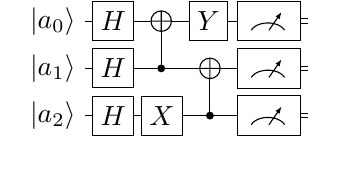
\begin{tikzpicture}
    \begin{yquant}
      qubit {$\ket{\reg_{\idx}}$} a[3];
      h a[0];
      h a[1];
      h a[2];
      cnot a[0] | a[1];
      x a[2];	
      y a[0];	 
      cnot a[1] | a[2]; 
      measure a[0-2];					 
     \end{yquant}
  \end{tikzpicture}
\caption{A example of quantum circuit}
\end{center}
\end{figure}

Each horizontal line represents each qubit and the square boxes that contain alphabets mean single quantum gates.  The sign which involves a vertical line means a CNOT gate, and the box on the most right side indicates measurement. 

\section{Quantum Entanglement}

Quantum entanglement is a special type of quantum state that cannot be described in the form of tensor product of the state of each particle.

\subsection{Bell Pair}
The entangled states between two qubits are called bell pairs, and each of four states has a special notation.
%% TODO: Add reference of EPR pair

\begin{equation}
  |\Phi^+\rangle = \frac{|00\rangle + |11\rangle}{\sqrt{2}}
  \end{equation}
  
  \begin{equation}
 |\Phi^-\rangle = \frac{|00\rangle - |11\rangle}{\sqrt{2}}
 \end{equation}
 
 \begin{equation}
 |\Psi^+\rangle = \frac{|01\rangle + |10\rangle}{\sqrt{2}}
 \end{equation}
 
 \begin{equation}
  |\Psi^-\rangle = \frac{|01\rangle - |10\rangle}{\sqrt{2}}
  \end{equation}.

\subsection{Multipartite Entanglement}
There are cases that more than two qubits are entangled and that state is called Greenberger–Horne–Zeilinger state or GHZ state.

Here is the braket notation of the GHZ state that involves three qubits.
\begin{equation}
  |GHZ\rangle = \frac{|000\rangle + |111\rangle}{\sqrt{2}}
\end{equation}.

In the general case, the braket notation of the GHZ state of N qubits is the following.
\begin{equation}
  |GHZ\rangle = \frac{|0\rangle^{\otimes N} + |1\rangle^{\otimes N}}{\sqrt{2}}
\end{equation}.

\subsection{Bell State Measurement}
Bell state measurement is a special type of quantum measurement that determines which bell pair the given two qubit entangled state is.
%% TODO: Add reference of BSM
\begin{figure}[ht]
  \begin{center}
    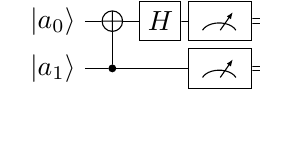
\begin{tikzpicture}
    \begin{yquant}
      qubit {$\ket{\reg_{\idx}}$} a[2];
      cnot a[0] | a[1];
      h a[0];	 
      measure a[0-1];					 
     \end{yquant}
  \end{tikzpicture}
\caption{Quantum circuit for bell state measurement}
\end{center}
\end{figure}

\begin{table}[ht]
  \begin{center}
    \begin{tabular}{|c|c|} \hline
      Measurement results & Bell state \\ \hline \cline{1-2}
      00 &  $|\Phi^+\rangle$ \\ \cline{1-2}
      01 & $|\Phi^-\rangle$ \\  \cline{1-2}
      10 &  $|\Psi^+\rangle$ \\ \cline{1-2}
      11 & $|\Psi^-\rangle$ \\  \hline  \cline{1-2}
    \end{tabular}
    \caption{A table of correspondence between measurement result and Bell pair}
  \end{center}
\end{table}

\subsection{Quantum Teleportation}

Unlike classical communication, quantum states cannot be just copied and transmit to other nodes due to the no-cloning theorem, which forbids duplication of any quantum state.  However, a method called quantum teleportation was proposed, which overcomes the restriction and allows sender to transmit single qubit state to a distant location. 
 		
This method requires both the single qubit state and a new Bell pair, and also the sender have to prepare two qubits and the receiver have to prepare one qubit.  After applying a CNOT gate and an H gate in the figure above, the sender have to measure both qubits and send those measurement results over the classical network.  After the receiver get those measurement results and apply some quantum gates if the measurement results of corresponding qubits on the sender's side are 1, in order to correct on the quantum state on the receiver's side.
%% TODO: Add reference of quantum teleportation (both idea and circuit)
%% TODO: Show that it works in the form of equations
%% TODO: Add reference of experimental works

\begin{figure}[ht]
  	\begin{center}
  		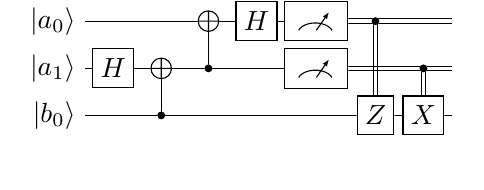
\begin{tikzpicture}
			\begin{yquant}
	 			qubit {$\ket{\reg_{\idx}}$} a[2];
	 			qubit {$\ket{\reg_{\idx}}$} b[1];
	 			h a[1];
        cnot a[1] | b[0];
	 			cnot a[0] | a[1];
        h a[0];	 
        measure a[0-1];	
        z b[0] | a[0];	
        x b[0] | a[1];				 
 			\end{yquant}
		\end{tikzpicture}
	\caption{Quantum circuit for quantum teleportation}
	\end{center}
\end{figure}

\newpage

\subsection{Entanglement Swapping}

Entanglement swapping is the method to extend quantum entanglement by performing joint measurement on several quantum entanglement.
For example, assume Alice has a single qubit, Bob has two qubits, and Charlie has one qubit. Then, there are Bell pairs between Alice's qubit and Bob's first qubit, and Bob's second qubit and Charlie's qubit, respectively.
If Bob performs Bell state measurement on both of his qubits, Alice's qubit and Charlie's qubit are eventually entangled, even though they have not interacted with each other.
This can be also seen as the teleporatation of a Bell pair by sending one of its particles.
Here is the figure of quantum circuit to perform entanglement swapping.
%% TODO: Add reference of entanglement swapping (both idea and circuit)
%% TODO: Show that it works in the form of equations
%% TODO: Add reference of experimental works

\begin{figure}[ht]
  \begin{center}
    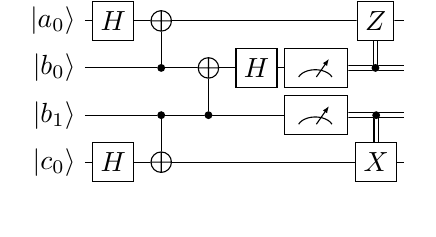
\begin{tikzpicture}
    \begin{yquant}
       qubit {$\ket{\reg_{\idx}}$} a[1];
       qubit {$\ket{\reg_{\idx}}$} b[2];
      qubit {$\ket{\reg_{\idx}}$} c[1];
       h a[0];
      h c[0];
       cnot a[0] | b[0];
       cnot c[0] | b[1];
      cnot b[0] | b[1];
      h b[0];	 
      measure b[0-1];	
      z a[0] | b[0];	
      x c[0] | b[1];		 
     \end{yquant}
  \end{tikzpicture}
\caption{Quantum circuit for entanglement swapping}
\end{center}
\end{figure}

\subsection{Entanglement Purification}
%% TODO: Add reference of entanglement purification (both idea and circuit)
%% TODO: Show that it works in the form of equations
%% TODO: Add reference of experimental works

Entanglement purification is a scheme to generate a set of quantum entanglements with higher fidelities from a larger set of imperfect quantum entanglements, local quantum operations, and classical communications.
This procedure is also called entanglement distillation, or quantum concatenation. This section presents an example of entanglement purification that generates a single bell pair with higher fidelity from two of those with less fidelity.

Assume Alice and Bob are supposed to share $|\Phi^+\rangle$, which is one of the Bell pairs. However, the state would be converted to the following mixed state due to the noisy nature of a quantum channel.
$$ \rho_{AB} = P_{\Phi^+}|\Phi^+\rangle\langle\Phi^+| + P_{\Phi^-}|\Phi^-\rangle\langle\Phi^-| + P_{\Psi^+}|\Psi^+\rangle\langle\Psi^+| + P_{\Psi^-}|\Psi^-\rangle\langle\Psi^-|$$

$$\sum_{s \in \{\Phi^+, \Phi^-, \Psi^+, \Psi^- \}} P_{s} = 1$$

Any mixed state can be converted to Werner state by applying Pauli operations and $\frac{\pi}{2}$ operations, so Alice and Bob can obtain the following state.

$$ \rho^{'}_{AB} = F|\Phi^+\rangle\langle\Phi^+| + \frac{1-F}{3}(|\Phi^-\rangle\langle\Phi^-| + |\Psi^+\rangle\langle\Psi^+| + |\Psi^-\rangle\langle\Psi^-|)$$

\begin{table}[ht]
  \begin{center}
    \begin{tabular}{|c|c|} \hline
      Before applying a CNOT gate & After a applying CNOT gate \\ \hline \cline{1-2}
      $|\Phi^+\rangle|\Phi^+\rangle$ &  $|\Phi^+\rangle|\Phi^+\rangle$ \\ \cline{1-2}
      $|\Phi^+\rangle|\Phi^-\rangle$ &  $|\Phi^-\rangle|\Phi^-\rangle$ \\ \cline{1-2}
      $|\Phi^+\rangle|\Psi^+\rangle$ &  $|\Phi^+\rangle|\Psi^+\rangle$ \\ \cline{1-2}
      $|\Phi^+\rangle|\Psi^-\rangle$ &  $|\Phi^-\rangle|\Psi^-\rangle$ \\ \cline{1-2}
      $|\Phi^-\rangle|\Phi^+\rangle$ &  $|\Phi^-\rangle|\Phi^+\rangle$ \\ \cline{1-2}
      $|\Phi^-\rangle|\Psi^-\rangle$ &  $|\Phi^+\rangle|\Phi^-\rangle$ \\ \cline{1-2}
      $|\Phi^-\rangle|\Psi^+\rangle$ &  $|\Phi^-\rangle|\Psi^+\rangle$ \\ \cline{1-2}
      $|\Phi^-\rangle|\Psi^-\rangle$ &  $|\Phi^+\rangle|\Psi^-\rangle$ \\ \cline{1-2}
      $|\Psi^+\rangle|\Phi^+\rangle$ &  $|\Psi^+\rangle|\Psi^+\rangle$ \\ \cline{1-2}
      $|\Psi^+\rangle|\Phi^-\rangle$ &  $|\Psi^+\rangle|\Psi^-\rangle$ \\ \cline{1-2}
      $|\Psi^+\rangle|\Psi^+\rangle$ &  $|\Psi^+\rangle|\Phi^+\rangle$ \\ \cline{1-2}
      $|\Psi^+\rangle|\Psi^-\rangle$ &  $|\Psi^+\rangle|\Phi^-\rangle$ \\ \cline{1-2}
      $|\Psi^-\rangle|\Phi^+\rangle$ &  $|\Psi^-\rangle|\Psi^+\rangle$ \\ \cline{1-2}
      $|\Psi^-\rangle|\Phi^-\rangle$ &  $|\Psi^-\rangle|\Psi^-\rangle$ \\ \cline{1-2}
      $|\Psi^-\rangle|\Psi^+\rangle$ &  $|\Psi^-\rangle|\Phi^+\rangle$ \\ \cline{1-2}
      $|\Psi^-\rangle|\Psi^-\rangle$ &  $|\Psi^-\rangle|\Phi^-\rangle$ \\ \cline{1-2}
    \end{tabular}
    \caption{A table of correspondence between Bell pairs before and after applying a CNOT gate}
  \end{center}
\end{table}

Two noisy bell pairs are required for entanglement purification, so assume the quantum state of the entire system can be described as follows.
\begin{multline*}
\rho^{'}_{a_1 b_1} \otimes \rho^{'}_{a_2 b_2} = F^2|\Phi^+\rangle|\Phi^+\rangle\langle\Phi^+|\langle\Phi^+| \\ 
+ \frac{F(1-F)}{3}(|\Phi^+\rangle|\Phi^-\rangle\langle\Phi^-|\langle\Phi^+|+|\Phi^+\rangle|\Psi^+\rangle\langle\Psi^+|\langle\Phi^+|+|\Phi^+\rangle|\Psi^-\rangle\langle\Psi^-|\langle\Phi^+| \\
+|\Phi^-\rangle|\Phi^+\rangle\langle\Phi^+|\langle\Phi^-|+|\Psi^+\rangle|\Phi^+\rangle\langle\Phi^+|\langle\Psi^+|+|\Psi^-\rangle|\Phi^+\rangle\langle\Phi^+|\langle\Psi^-|) \\ 
+ \frac{(1-F)^2}{9}(|\Phi^-\rangle|\Phi^-\rangle\langle\Phi^-|\langle\Phi^-|+|\Phi^-\rangle|\Psi^+\rangle\langle\Psi^+|\langle\Phi^-|+|\Phi^-\rangle|\Psi^-\rangle\langle\Psi^-|\langle\Phi^-| \\
+ |\Psi^+\rangle|\Phi^-\rangle\langle\Phi^-|\langle\Psi^+|+|\Psi^+\rangle|\Psi^+\rangle\langle\Psi^+|\langle\Psi^+|+|\Psi^+\rangle|\Psi^-\rangle\langle\Psi^-|\langle\Psi^+| \\
+|\Psi^-\rangle|\Phi^-\rangle\langle\Psi^-|\langle\Phi^-|+|\Psi^-\rangle|\Psi^+\rangle\langle\Psi^+|\langle\Psi^-|+|\Psi^-\rangle|\Psi^-\rangle\langle\Psi^-|\langle\Psi^-|)
\end{multline*}

One of the bell pair $\rho^{'}_{a_1 b_1}$ is called source bell pair, which may be purified, and the other one $\rho^{'}_{a_2 b_2}$  is called target bell pair, which is going to be measured. Then, Alice and Bob perform CNOT operations between $a_1$ and $a_2$, and $b_1$ and $b_2$, respectively.
The entire quantum state on this point would be as follows.
\begin{multline*}
  \rho^{'}_{a_1 b_1} \otimes \rho^{'}_{a_2 b_2} = F^2|\Phi^+\rangle|\Phi^+\rangle\langle\Phi^+|\langle\Phi^+| \\ 
  + \frac{F(1-F)}{3}(|\Phi^-\rangle|\Phi^-\rangle\langle\Phi^-|\langle\Phi^-|+|\Phi^+\rangle|\Psi^+\rangle\langle\Psi^+|\langle\Phi^+|+|\Phi^-\rangle|\Psi^-\rangle\langle\Psi^-|\langle\Phi^-| \\
  +|\Phi^-\rangle|\Phi^+\rangle\langle\Phi^+|\langle\Phi^-|+|\Psi^+\rangle|\Psi^+\rangle\langle\Psi^+|\langle\Psi^+|+|\Psi^-\rangle|\Psi^+\rangle\langle\Psi^+|\langle\Psi^-|) \\ 
  + \frac{(1-F)^2}{9}(|\Phi^+\rangle|\Phi^-\rangle\langle\Phi^-|\langle\Phi^+|+|\Phi^-\rangle|\Psi^+\rangle\langle\Psi^+|\langle\Phi^-|+|\Phi^+\rangle|\Psi^-\rangle\langle\Psi^-|\langle\Phi^+| \\
  + |\Psi^+\rangle|\Psi^-\rangle\langle\Psi^-|\langle\Psi^+|+|\Psi^-\rangle|\Phi^+\rangle\langle\Phi^+|\langle\Psi^+|+|\Psi^+\rangle|\Psi^-\rangle\langle\Psi^-|\langle\Psi^+| \\
  +|\Psi^-\rangle|\Psi^-\rangle\langle\Psi^-|\langle\Psi^-|+|\Psi^-\rangle|\Phi^+\rangle\langle\Phi^+|\langle\Psi^-|+|\Psi^-\rangle|\Phi^-\rangle\langle\Phi^-|\langle\Psi^-|)
  \end{multline*}

After that, they measure $a_2$ and $b_2$ respectively, which is the qubit on the target bell pair on their side and exchange the measurement results.  

If their measurement results match, the purification is successful, while they have to discard the source bell pair and try again if those results do not match.

Here is the quantum state after measuring the target bell pair.

\begin{multline*}
\rho^{'}_{ab} = \frac{1}{N} \big[ F^2 + \frac{1}{9}\big(1-F \big)^2\big]|\Phi^+\rangle\langle\Phi^+| + \frac{2F(1-F)}{3N}|\Phi^-\rangle\langle\Phi^-| + \frac{2(1-F)^2}{9N}(|\Psi^+\rangle\langle\Psi^+| + |\Psi^-\rangle\langle\Psi^-|) \\
(N = F^2 + \frac{2F(1-F)}{3} + \frac{2(1-F)^2}{9})
\end{multline*}

The purification becomes successful if F  $> \frac{1}{2}$

\section{Quantum Networking}
\subsection{Quantum Node}
\subsection{Quantum Repeater}
\subsection{Quantum Link}
\subsection{Major Applications of Quantum Networking}


\chapter{Problem Definition}
\label{problem-definition}

\section{Problem Definition}

In order to maximize the overall performance and the aggregative use of resource in the entire network, several connections are desired to be established in the real-time fashion.
However, there are two major obstacles to overcome in the case of quantum network. 

One is the absence of link management protocol for quantum network. There is a previous work \cite{aparicio2011multiplexing} that proposes and compares the performance of various multiplexing strategies, but it does not mention any concrete methods to establish multiple connections and allocate the available physical links to each of these connections.

The other one is the lack of interaction between connection management and the subsequent resource management. The current RuleSet-based communication protocol \cite{matsuo2019quantum} only proposes the scheme to establish a single connection and it does not explain the method to tear it down and free the allocated physical links after the end of RuleSet execution. 

This thesis tackles the first problem by proposing the link management protocol the involves the negotiation about the set of connections to establish and the one about when to start the establishment. It also discuss the messages and their properties that are required to run this protocol.

Additionally, this thesis explains how the link management scheme is going to be triggered when a new connection is established and the old one is torn down. This explanation includes the methods to implement in the relevant software components when RuleSet-based quantum network is simulated or deployed in the real world.
%%% Local Variables:
%%% mode: japanese-latex
%%% TeX-master: "./thesis"
%%% End:

\chapter{Proposal: Link Management For Quantum Network}
\label{proposal}

\section{Overview}

This chapter proposes the protocol for the management of the physical Bell pairs that are available on each quantum link.

This protocol has two separated phases. The first phase is the negotiation about the set of RuleSets that are going to be established in the next round. The second phase is the negotiation about when to apply the next set of RuleSets.
These negotiations will take place between the two end point of each link.

\section{Link Allocation Policy}

In order to establish multiple connections over a single link, the both end nodes of the link need to make the coordinated decisions about what connections need to be established.
This set of connections, to be more specific, the set of RuleSets, would be called \textbf{Link Allocation Policy} in the rest of this thesis.

\section{Link Allocation Policy Negotiation Phase}

After the node receives a message that notifies the establishment of a new connection, or the termination of one of the existing connections, both nodes between a single link need to agree with the link allocation policy that are going to be executed in the next round.
Therefore, this protocol involves the transmission of messages that include the information of the next link allocation policy in each node.  It has to be mentioned that the order of arrival of RuleSets in the next policy might be different, so the protocol also requires the mechanism to determine which policy needs to be prioritized.
This can be achieved by inserting a random integer to the message and adopt the order with the larger value.

\section{The Timing Negotiation Phase}

The end nodes of a physical link also need to align the timing of updating the link policy in order to assign the same Bell pair to the connection.
Otherwise,they might allocate the physical qubits of two different Bell pairs, which might end up with the failure of the entire connection.

\section{Resource Management}

The actual resource allocation process needs to take place before or during the execution of the RuleSets that were determined in the previous steps.
On the contrary to that, the release of physical resources that were allocated to the terminated RuleSets need to be executed after the notification of connection teardown, which the node receives from the networking layer.

\section{Messages}

This protocol involves the exchange of two kinds of messages, which are \textbf{LinkAllocationUpdateMessage} and \textbf{BarrierMessage}.
This section proposes the required fields and their types in each message.

\subsection{LinkAllocationUpdateMessage}
 
This message contains the following fields.

\begin{table}[ht]
  \begin{center}
    \begin{tabular}{|m{10em}|m{10em}|m{10em}|} \hline
      Field Name & Type & Explanation \\ \hline \cline{1-3}
      srcAddress & integer & The source address \\ \cline{1-3}
      destAddress & integer & The destination address \\ \cline{1-3}
      activeLinkAllocations & unsigned long [] & The array of IDs of the RuleSets in the active link allocation policy \\ \cline{1-3}
      nextLinkAllocations & unsigned long [] & The array of IDs of the RuleSets in the upcoming link allocation policy \\ \cline{1-3}
      randomValue & integer & A random value \\ \cline{1-3}
    \end{tabular}
    \caption{The Message Fields in a LinkAllocationUpdateMessage}
  \end{center}
\end{table}

\subsection{BarrierMessage}

This message contains the following fields.

\begin{table}[ht]
  \begin{center}
    \begin{tabular}{|c|c|c|} \hline
      Field Name & Type & Explanation \\ \hline \cline{1-3}
      srcAddress & integer & The source address \\ \cline{1-3}
      destAddress & integer & The destination address \\ \cline{1-3}
      sequenceNumber & integer & A sequence number of the first available physical Bell Pair \\ \cline{1-3}
    \end{tabular}
    \caption{The Message Fields in a BarrierMessage}
  \end{center}
\end{table}

\newpage

\section{Finite State Machine For Link Allocation Policy}

Finite state machine (FSM) is commonly provides a simple and clear description about the behavior of the communication protocol \cite{BOCHMANN1978361}.
Each state in the finite state machine represents the condition of a communication node, its events represents the change such as transmission and reception of messages, and the action represents the reaction to the event based on the previous condition.
This section explains the behavior of one of the end nodes of a link during the negotiation phase. 

\subsection{States}

\subsubsection{Init}
This is the initial state that each node starts with.  
In this state, neither the negotiation about the upcoming link allocation policy or the one about when to update the policy are happening.
The FSM transits into either IncomingLAUWait state or LAUNotSent state by sending an LinkAllocationUpdateMessage or receiving the one from its neighboring nodes.

\subsubsection{IncomingLAUWait}
This is the state when a node sends a LinkAllocationUpdateMessage to its neighboring node. 
In this state, a node is waiting for the incoming LinkAllocationUpdateMessage from those nodes in return, 
so that the FSM can move to SyncNextPolicy state by coordinating the new link allocation policy.

\subsubsection{LAUNotSent}
This is the state when a node receives a LinkAllocationUpdateMessage from its neighboring node. 
In this state, a node is about to send LinkAllocationUpdateMessages back to those nodes, so that the FSM can move to SyncNextPolicy state by coordinating the new link allocation policy.

\subsubsection{SyncNextPolicy}
This is the state when both end nodes coordinated the next link allocation policy.
The FSM transits into either BarrierNotSent state or IncomingBarrierWait state if the negotiation goes successfully, otherwise it transits back to Init if they fail.

\subsubsection{IncomingBarrierWait}
This is the state when a node sends a BarrierMessage to its neighboring node. 
In this state, a node is waiting for the incoming BarrierMessage from that node in return, 
so that the FSM can move to BarrierMessage state by coordinating from which Bell Pair the new link allocation policy should be applied.

\subsubsection{BarrierNotSent}
This is the state when a node receives a BarrierMessage from its neighboring node. 
In this state, a node is about to send BarrierMessage back to that node, 
so that the FSM can move to SyncNextSeqNum state by coordinating from which Bell Pair the new link allocation policy should be applied.

\subsubsection{SyncNextSeqNum}
This is the state when both end nodes of a link successfully coordinated from which Bell Pair the new link allocation policy will be updated.
The FSM transits to the Init state until the next negotiation about the link allocation policy becomes triggered from the networking layer.

\subsection{Events}

\subsubsection{TxLAU}
This event indicates the transmission of a LinkAllocationUpdateMessage.

\subsubsection{RxLAU}
This event indicates the reception of a LinkAllocationUpdateMessage.

\subsubsection{TxBr}
This event indicates the transmission of a BarrierMessage.

\subsubsection{RxBr}
This event indicates the reception of a BarrierMessage.

\subsubsection{LAUSuccess}
This event indicates the success in the coordination of the next link allocation policy.

\subsubsection{LAUFail}
This event indicates the failure in the coordination of the next link allocation policy.


\subsubsection{BarrierSuccess}
This event indicates the success in the coordination of the first sequence number that the new link allocation policy is applied.

\subsubsection{BarrierFail}
This event indicates the failure in the coordination of the first sequence number that the new link allocation policy is applied.

\newpage

\subsection{Description of Finite State Machine}

\begin{figure}[ht] % ’ht’ tells LaTeX to place the figure ’here’ or at the top of the page
  \centering % centers the figure
  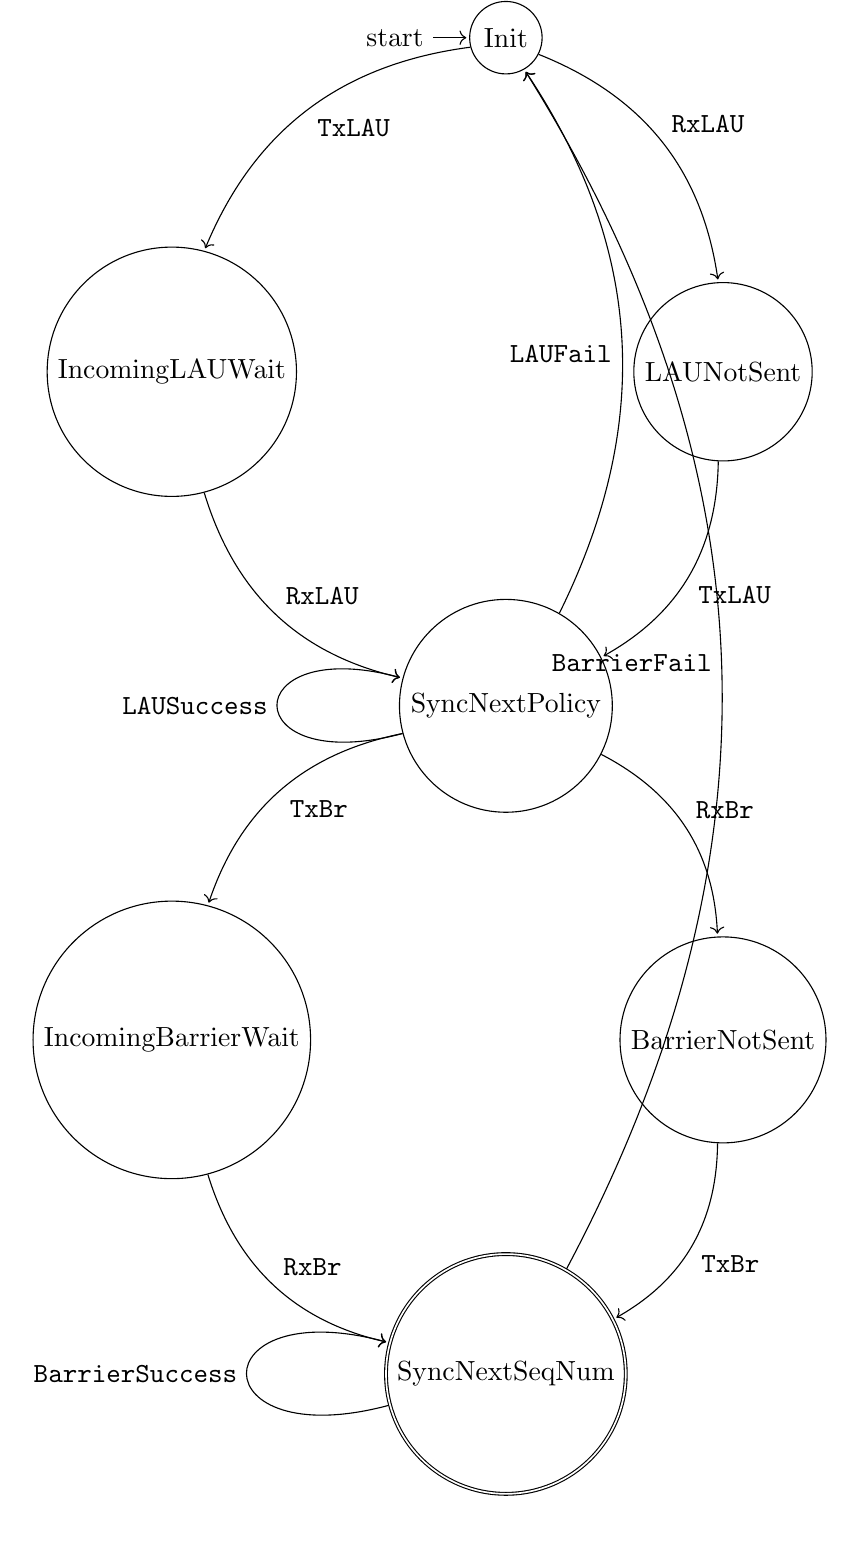
\begin{tikzpicture}[shorten >=1pt,node distance=6cm,on grid,auto]
    \node[state, initial] (Init) {Init};
    \node[state, below left of=Init] (IncomingLAUWait) {IncomingLAUWait};
    \node[state, right of=IncomingLAUWait, xshift=1cm] (LAUNotSent) {LAUNotSent};
    \node[state, below right of=IncomingLAUWait] (SyncNextPolicy) {SyncNextPolicy};
    \node[state, below left of=SyncNextPolicy] (IncomingBarrierWait) {IncomingBarrierWait};
    \node[state, right of=IncomingBarrierWait, xshift=1cm] (BarrierNotSent) {BarrierNotSent};
    \node[state, accepting, below right of=IncomingBarrierWait] (SyncNextSeqNum) {SyncNextSeqNum};

   \draw[->] (Init) edge [bend right] node {\tt TxLAU} (IncomingLAUWait);
   \draw[->] (Init) edge [bend left] node {\tt RxLAU} (LAUNotSent);
   \draw[->] (IncomingLAUWait) edge [bend right] node {\tt RxLAU} (SyncNextPolicy);
   \draw[->] (LAUNotSent) edge [bend left] node {\tt TxLAU} (SyncNextPolicy);
   \draw[->] (SyncNextPolicy) edge [bend right] node {\tt TxBr} (IncomingBarrierWait);
   \draw[->] (SyncNextPolicy) edge [bend left] node {\tt RxBr} (BarrierNotSent);
   \draw[->] (SyncNextPolicy) edge [loop left] node {\tt LAUSuccess} ();
   \draw[->] (SyncNextPolicy) edge [bend right] node {\tt LAUFail} (Init);
   \draw[->] (IncomingBarrierWait) edge [bend right] node {\tt RxBr} (SyncNextSeqNum);
   \draw[->] (BarrierNotSent) edge [bend left] node {\tt TxBr} (SyncNextSeqNum);
   \draw[->] (SyncNextSeqNum) edge [loop left] node {\tt BarrierSuccess} ();
   \draw[->] (SyncNextSeqNum) edge [bend right] node {\tt BarrierFail} (Init);

  \end{tikzpicture}
  \caption{The FSM for the negotiation phase}
  \label{fig:my_label}
\end{figure}

\section{Finite State Machine For Link Management}

This section provides the different finite state machine for the link management phase. It focuses on the behavior of a single Bell pair that exists on the quantum link for simplicity.

\subsection{States}

\subsubsection{Up}
This is the state when a physical Bell pair is established on a quantum link between its two end nodes. In this state, it is not allocated to any specific RuleSet.
The FSM transits to Allocated if the link becomes allocated to one of the RuleSets in the active link allocation policy.

\subsubsection{Down}
This is the state when a physical Bell pair on a quantum link is not established between its two end nodes. In this state, it can be no Bell pair between two existing quantum memories in the case of a quantum repeaters with those memories, or the situation when incoming photons have not arrived to memoryless quantum repeaters.
The FSM transits to Up if a Bell pair is established.

\subsubsection{Allocated}
This is the state when a physical Bell pair is allocated to one of the RuleSets in the active link allocation policy.
The FSM transits to Up if the link becomes released after the connection that this link used to be allocated is terminated.
It can also transits to Down if the physical qubits on the link are measured during execution of the RuleSet that this link is allocated to.

\subsection{Events}

\subsubsection{BellPairGen}
This event indicates the generation of a Bell pair

\subsubsection{Allocate}
This event indicates the allocation of a given Bell pair to RuleSet.

\subsubsection{Free}
This event indicates the release of an available Bell pair from that RuleSet that it is used to be allocated to.

\subsubsection{Measure}
This event indicates the measurement of two physical qubits of the given Bell pair while the RuleSet is being executed.

\subsection{Description of Finite State Machine}

\begin{figure}[ht] % ’ht’ tells LaTeX to place the figure ’here’ or at the top of the page
  \centering % centers the figure
  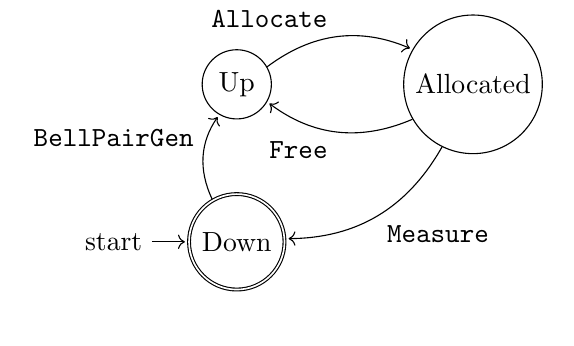
\begin{tikzpicture}[shorten >=1pt,node distance=3cm,on grid,auto]
    \node[state] (Up) {Up};
    \node[state, initial, accepting, below = 2cm of Up] (Down) {Down};
    \node[state, right = 3cm of Up] (Allocated) {Allocated};

    \draw[->] (Down) edge [bend left] node {\tt BellPairGen} (Up);
    \draw[->] (Up) edge [bend left] node {\tt Allocate} (Allocated);
    \draw[->] (Allocated) edge [bend left] node {\tt Free} (Up);
    \draw[->] (Allocated) edge [bend left] node {\tt Measure} (Down);
  \end{tikzpicture}
  \caption{The FSM for the resource management phase}
  \label{fig:my_label}
\end{figure}


%%% Local Variables:
%%% mode: japanese-latex
%%% TeX-master: "../bthesis"
%%% End:

\chapter{Simulation}
\label{simulation}

\section{QuISP (Quantum Internet Simulation Package)}

\subsection{Overview}

QuISP \cite{satoh2022quisp} is a quantum network simulator which aims to simulate the behavior of a large-scale quantum network. It is built on top of OMNeT++ \cite{10.5555/1416222.1416290}, which is an event-driven network simulator.
The reason why QuISP is built on top of OMNet++ is that OMNet++ allows users to define their own networking layers.
QuISP can simulate various types of errors, not only Pauli X error, Pauli Y error and Pauli Z error, but also relaxation error and excitation error.
Physical noise on an actual quantum system with $n$ qubits are usually simulated in the form of a density matrix, which would includes $2^n \times 2^n$ elementss and soon becomes intractable as $n$ becomes larger.
QuISP realizes the scalable simulation of quantum network by simulating the physical error using an error probability vector, which would take the following form.

\begin{equation}
  \overrightarrow{\pi}(t) = (\pi_I, \pi_X, \pi_Y, \pi_Z, \pi_R, \pi_E, \pi_L)
\end{equation}
It contains $m+1$ elements (m is the number of simulated error types)
The time evolution of error probability vector is provided by a transition error matrix $Q$.
\begin{equation}
  \overrightarrow{\pi}(t) = \overrightarrow{\pi}(t-1)Q 
\end{equation}

The error probability vector above is the one for a single qubit, so the one for $N$ qubit system contains $N(m+1)$ elements.

\subsection{Hardware Components}

Communication between two quantum nodes is achieved by transmission of photons via an optical fiber, and the fiber is mocked by an object called quantum link.
QuISP supports three main link architecture. 

\subsubsection{Memory-Memory}
The first one is Memory-Memory that two nodes are directly connected via a quantum link and the Bell State Analyzer is equipped in the receiver node.

\subsubsection{Memory-Interface-Memory}
The second one is Memory-Interface-Memory. Both end nodes of a quantum link emits photons to Bell State Analyzer located in the middle. After they become entangled, all the measurements results and required operations are sent back to both nodes.

\subsubsection{Memory-Source-Memory}
The last one Memory-Source-Memory. All the entanglement pairs are both generated and sent from the source of entangled photonic pair states in the middle.

\subsection{Software Components}

\subsubsection{Connection Manager}

Connection establishment is done when connection manager at the Initiator nodes sends ConnectionSetupRequest to the Responder node and intermediate nodes sends additional information such as those about QNIC.
After that, the connection manager at the responder node sends ConnectionSetupResponse to each node along the path of the connection.

\subsubsection{Hardware Monitor}
Hardware monitor is the module that collects the information of a quantum link such as fidelity and generation rate and pass those information to the routing daemon and the connection manager.

\subsubsection{Bell Pair Store}
Bell pair store is the module that stores the entanglement pairs generated from a support node such as a Bell State Analyzer.

\subsubsection{Rule Engine}
Rule engine is the component that is in charge for executing the given RuleSets and monitor the conditions of physical qubits.

\subsubsection{Real-Time Controller}
Real-time controller is the component that is responsible for the initialization of physical components and coordination of the timing for photon emission.

\subsubsection{Routing Daemon}
Routing daemon is the component that generates and exchanges the routing table for quantum network interface card, or QNIC in short.

\section{Implementation}

\subsection{RuleEngine}
\subsection{Link Allocation Policy Negotiation}
\subsubsection{Link Allocation Timing Negotiation}
\subsubsection{Resource Allocation}


%%% Local Variables:
%%% mode: japanese-latex
%%% TeX-master: "../bthesis"
%%% End:

\chapter{Related Works}
\label{related works}

\section{Protocol Stack For Quantum Network}

This section discusses the protocol stack for quantum network. The protocol stack is a collection protocols that supports various levels of communication.
Here is the comparison of the protocol stack for quantum network that are presented in the previous works.

\begin{table}[ht]
  \begin{center}
    \begin{tabular}{|c|c|} \hline
       Name & Functionality \\ \hline \cline{1-2}
       Application & Run an application on an E2E connection \\ \hline \cline{1-2}
       Purification Control & Perform purification to E2E connection \\ \hline \cline{1-2}
       Entanglement Swapping Control & Perform entanglement swapping to establish an E2E connection \\
       Purification Control & Perform purification to a physical bell pair \\ \hline \cline{1-2} \hline \cline{1-2}
       Entanglement Control & Provide robustness to the bell pair establishment \\ \hline \cline{1-2} \hline \cline{1-2}
       Physical Entanglement & Establish a physical bell pair \\ \hline \cline{1-2} \hline \cline{1-2}
    \end{tabular}
    \caption{Protocol Stack for Quantum Network in \cite{Van_Meter_2009}}
  \end{center}
\end{table}

The work \cite{Van_Meter_2009} is the first study that proposed the quantum protocol stack and its proposal assumes the quantum repeater protocol that manages error using entanglement purification for both a link between two neighboring nodes and an end-to-end connection between two end nodes.
It has to be mentioned that this work assumes the number of hops for entanglement swapping and purification is assumed to be $N = 2^n$ ($n$ is a positive integer) in a linear topology. Also, this work does not assume the routing functionality in any protocol layer.

\begin{table}[ht]
  \begin{center}
    \begin{tabular}{|c|c|} \hline
      Name & Functionality \\ \hline \cline{1-2}
      Application & Run an application on an E2E connection \\ \hline \cline{1-2}
      Transport & Qubit transmission \\ \hline \cline{1-2}
      Network & Long distance entanglement \\ \hline \cline{1-2}
      Link & Robust entanglement generation \\ \hline \cline{1-2}
      Physical & Attempt entanglement generation \\ \hline \cline{1-2}
    \end{tabular}
    \caption{Protocol Stack for Quantum Network in \cite{Dahlberg_2019}}
  \end{center}
\end{table}

Another work \cite{Dahlberg_2019} proposes the different stack of quantum networking protocols that assumes the existence of transport layer that teleports a qubit using an end-to-end connection that is established by up to the network layer.
Also, it mentions the future outlook that the functionalites of routing and entanglement management may be separated from the network layer.

Although several previous works present different protocol stacks in terms of those in the upper layer, those protocol stacks still have some common features, which are 
\begin{itemize}
  \item Establishment of an actual physical Bell pair
  \item Robust entanglement generation
  \item Extension of physical bell pairs in order to establish an end-to-end Bell pair
\end{itemize}

These three elements will be the foundation of quantum network. This thesis will introduce specific protocols in the physical layer that is responsible for establishing the physical bell pair and link layer that adds robustness in the process of entanglement generation.

\section{Physical Layer Protocols For Quantum Network}

A previous work \cite{Dahlberg_2019} proposes the communication protocol for the physical layer for two of the four different use cases of a quantum network that it defines.
The protocol is called the midpoint heralding protocol (MHP) in short.

\subsubsection{MHP for Create and Keep (CK)}

Create and Keep is the use case when multiple entanglements should be stored simultaneously, such as quantum sensing \cite{PhysRevLett.109.070503}, metrology \cite{komar2014quantum} and distributed quantum computing \cite{10.1145/1060590.1060662}.
The process of entanglement generation is triggered by the reception of the message from the link layer, which includes the following parameters.
\begin{itemize}
  \item An ID for the entanglement generation attempt
  \item Generation parameters
  \item Qubits on the physical device which entanglements will be stored.
  \item The detail of microwave and laser pulse sequence
\end{itemize}

Then, the GEN message, which asks for the entanglement generation with the ID in the given message and the timestamp is sent to the support node in the middle. 
The support node uses the given timestamp to see if it receives the same IDs from the both side within a certain amount of time.
Also, it sends a REPLY message which includes the result, which is either success or failure, the generated state, and a sequence of IDs of entangled qubits after the measurement.
Then the end node performs an additional gate operation on the physical qubit depending on what state is generated, and redirected the received information to the link layer.

\subsubsection{MHP for Measure Directly (MD)}

Measure Directly is the usecase when multiple entanglements need to be created sequentially such as quantum key distribution \cite{PhysRevLett.67.661} and secure identification \cite{damgaard2007secure}.
The basic procedure is the same as the one above, but there are two main differences.  One is the operations that the end nodes perform on qubits.
Instead of performing additional state, it performs measurement on a specific basis.  The othe one is the timing of measurement. These nodes perform these measurement only they receive successful responses.

\section{Link Layer Protocols For Quantum Network}

Communication protocols for link layer have been proposed in several previous studies \cite{Van_Meter_2009,Dahlberg_2019,matsuo2019simulation}.
The biggest difference between the communication protocol for the physical layer protocol and the one for the link layer is reliability.
The former involves the process of actual entanglement generation and classical communication that triggers the process. On the other hand, the latter requires the additional classical communication that indicates the beginning and end of entanglement generation.

The first protocol \cite{Van_Meter_2009} assumes that end nodes of a physical link are directly connected via an optical fiber. First of all, multiplexed optical pulses are sent to the receiver and they are demultiplexed and measured at the receiver.
After several entanglements are generated, the ACK or NACK "keep" flags for each physical qubit are sent back to the sender.
\begin{figure}[H]
  \centerline{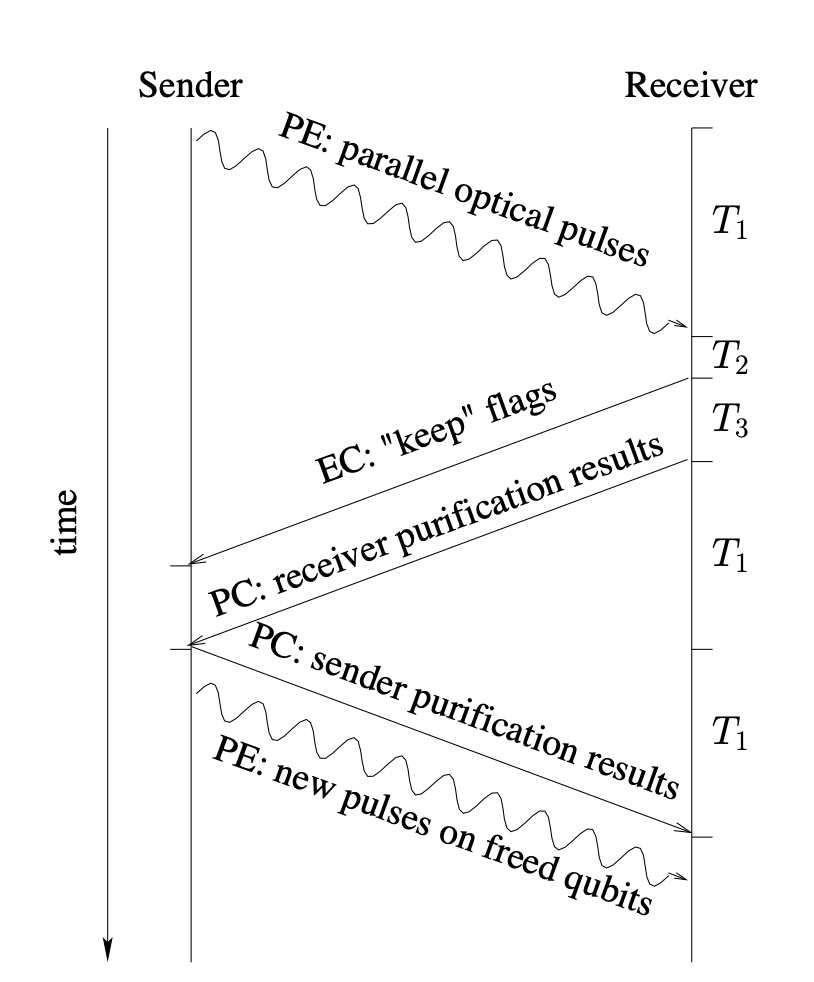
\includegraphics[width=.5\columnwidth]{images/link_protocol_rdv.jpg}}
  \caption{Message sequences in the link layer protocol in  \cite{Van_Meter_2009}}
\end{figure}

The next protocol \cite{Dahlberg_2019} assumes several components, which are Distributed Queue to store requests, Quantum Memory Management (QMM) to decide which physical qubits to use, Fidelity Estimation Unit (FEU) to estimate hardware capabilities, and Scheduler that schedules the timing of incoming requests.
The link layer receives a CREATE operation from the upper networking layer with the number of entangled pairs it requires, the minimum required fidelity, and the amount of time it can wait.
After that, the FEU estimates the hardware capabilities and the amount of time it would take to generate the entanglement pairs.  It the request will be rejected if the estimated time exceeds the given amount of time.
If it is accepted, the link layer send the "yes" response with the unique ID and the number of requested entanglement pairs.

\begin{figure}[H]
  \centerline{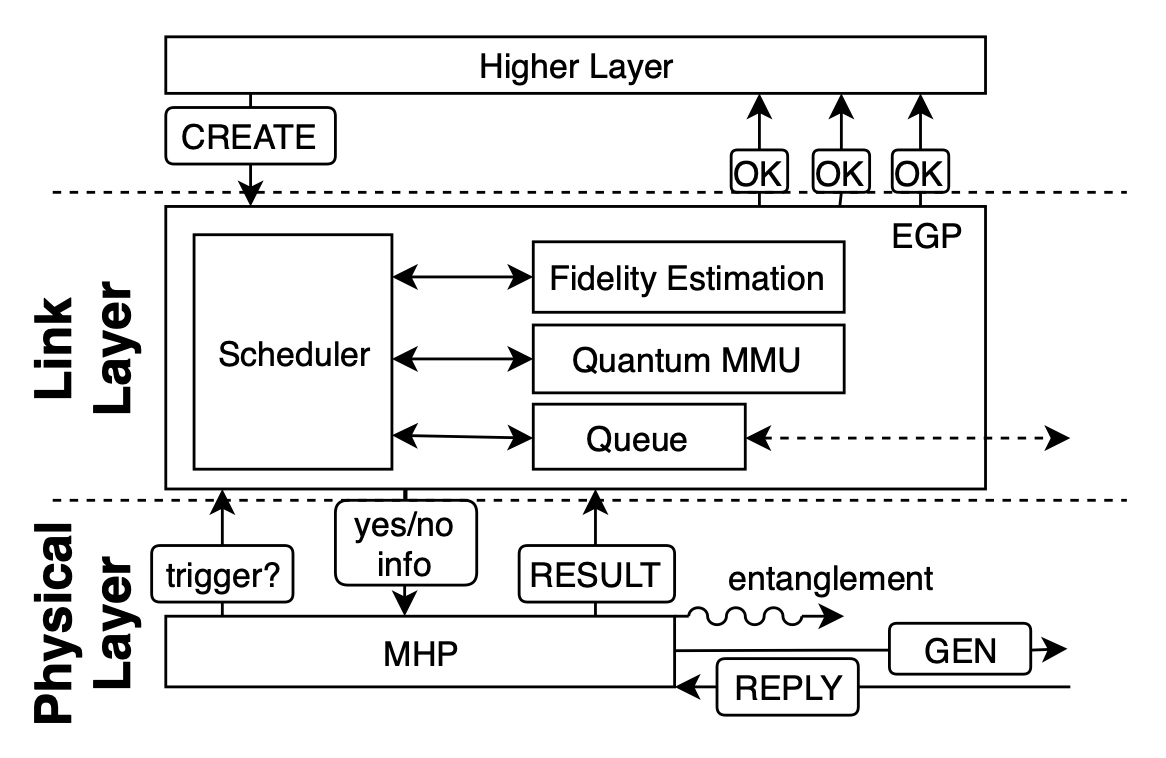
\includegraphics[width=.5\columnwidth]{images/link_protocol_dahlberg.png}}
  \caption{Message sequences in the link layer protocol in  \cite{Dahlberg_2019}}
\end{figure}

The last protocol \cite{matsuo2019simulation} assumes either SendReceiver or MeetInTheMiddle for its link architecture. First of all, each end node sends Boot Up Notification to its neighboring BSA nodes.
After these notifications are received, the BSA node in the middle calculates the emission timing and send it back to its neighboring end nodes.
Then end nodes emit a bulk of photons and send the message to notify the end of photon emission.
Lastly, the BSA node transmits the measurement results either sequentially or in batch and the message that includes the next emission timing.
\begin{figure}[H]
  \centerline{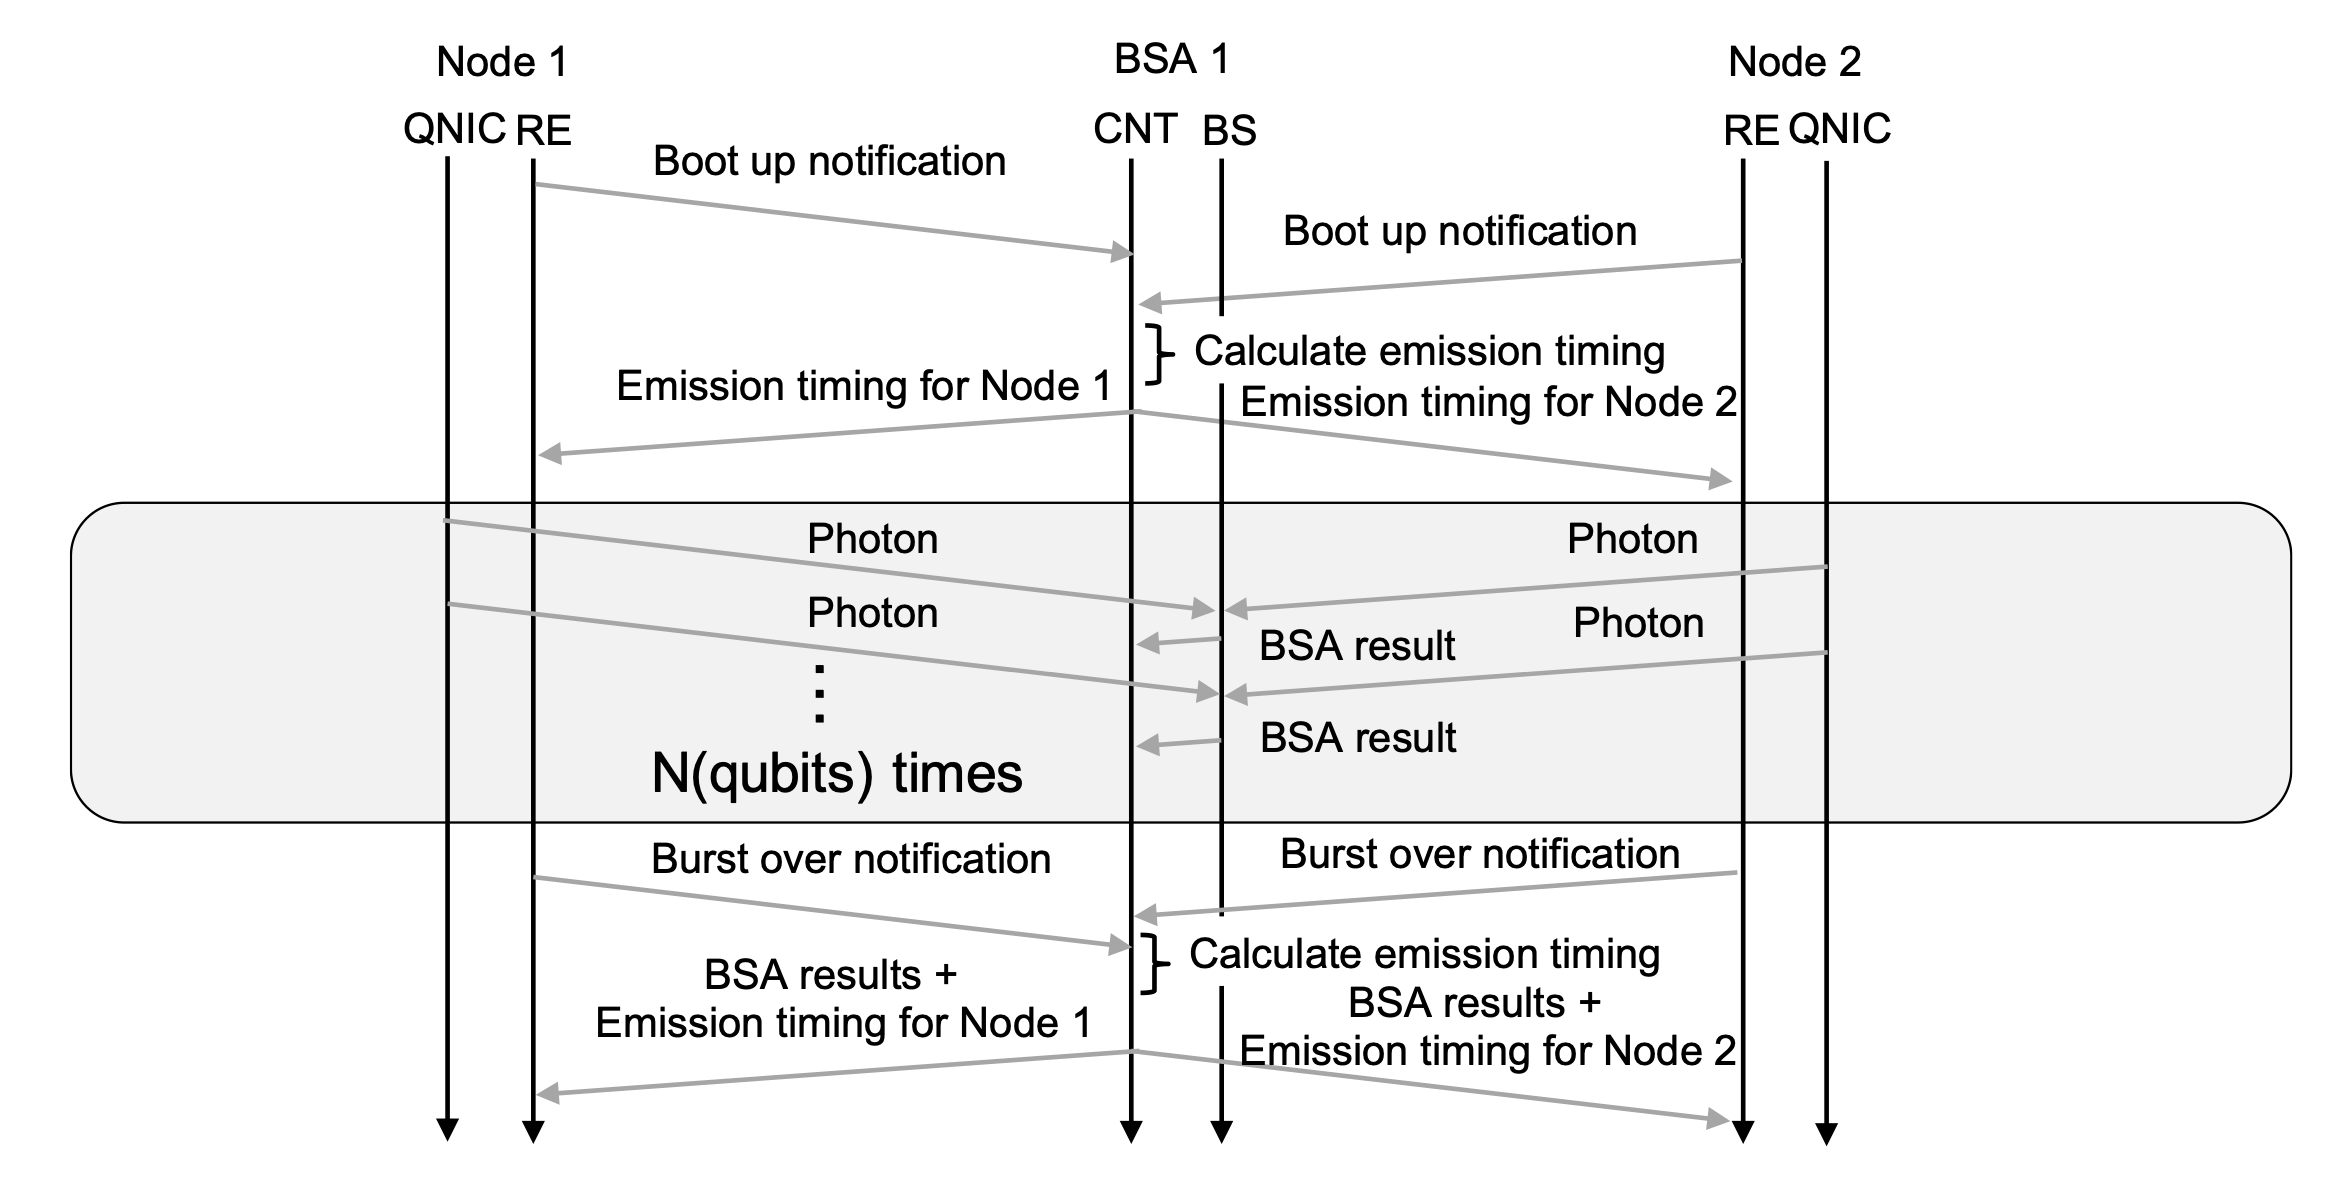
\includegraphics[width=.5\columnwidth]{images/link_protocol_matsuo.png}}
  \caption{Message sequences in the link layer protocol in \cite{matsuo2019simulation}}
\end{figure}

\section{RuleSet-Based Quantum Network}

This section explains the essential features of RuleSet-based quantum networking. Before the connection is established, the initiator sends the ConnectionSetupRequest and the information about each link along the path to the responder.
After the responder receives the request, it sends the ConnectionSetupResponse and an object called RuleSet.
RuleSet is a collection of Rule, which contains both one or more Condition clauses and Action clause. Condition clause is the condition to meet in order to perform a specific operation, and an Action clause is the operation itself, such as entanglement swapping and purification.
Connection establishment is performed by executing the RuleSet in each node instead of performing synchronization with neighboring nodes for each operation, so that it can reduce the number of message exchange and eventually build a more scalable quantum network.

\begin{figure}[H]
  \centerline{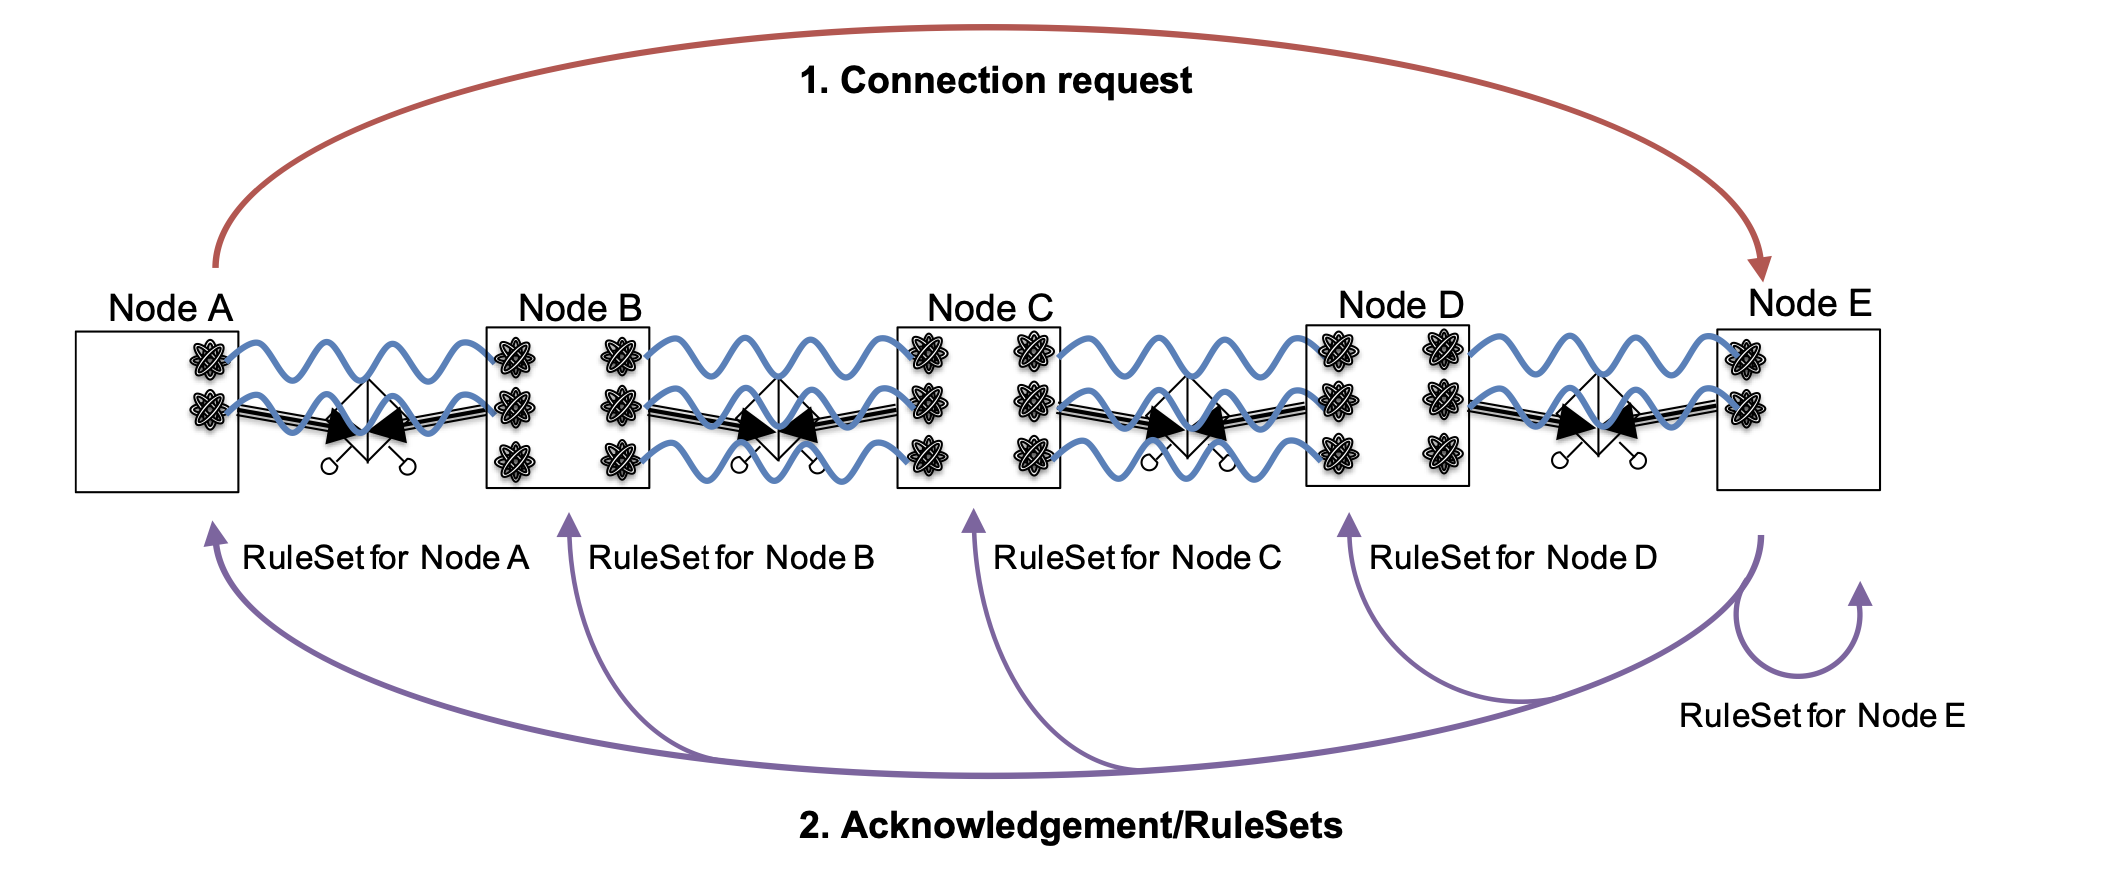
\includegraphics[width=.5\columnwidth]{images/ruleset_connection.png}}
  \caption{Connection Setup in the RuleSet-based quantum network from \cite{matsuo2019simulation}}
\end{figure}




\chapter{Evaluation}
\label{evaluation}
hoge

\section{Experiment}



%%% Local Variables:
%%% mode: japanese-latex
%%% TeX-master: "./thesis"
%%% End:

\chapter{Conclusion}
\label{conclusion}

hoge

\section{Conclusion}

\section{Future Works}

%%% Local Variables:
%%% mode: japanese-latex
%%% TeX-master: "../thesis"
%%% End:

% \appendix
\chapter{Appendix}


\section{The Entire Calculation To Derive The Bell Pair After Purification}
\label{appendix:purification}

\begin{table}[ht]
  \begin{center}
    \begin{tabular}{|c|c|} \hline
      Before applying a CNOT gate & After a applying CNOT gate \\ \hline \cline{1-2}
      $|\Phi^+\rangle|\Phi^+\rangle$ &  $|\Phi^+\rangle|\Phi^+\rangle$ \\ \cline{1-2}
      $|\Phi^+\rangle|\Phi^-\rangle$ &  $|\Phi^-\rangle|\Phi^-\rangle$ \\ \cline{1-2}
      $|\Phi^+\rangle|\Psi^+\rangle$ &  $|\Phi^+\rangle|\Psi^+\rangle$ \\ \cline{1-2}
      $|\Phi^+\rangle|\Psi^-\rangle$ &  $|\Phi^-\rangle|\Psi^-\rangle$ \\ \cline{1-2}
      $|\Phi^-\rangle|\Phi^+\rangle$ &  $|\Phi^-\rangle|\Phi^+\rangle$ \\ \cline{1-2}
      $|\Phi^-\rangle|\Psi^-\rangle$ &  $|\Phi^+\rangle|\Phi^-\rangle$ \\ \cline{1-2}
      $|\Phi^-\rangle|\Psi^+\rangle$ &  $|\Phi^-\rangle|\Psi^+\rangle$ \\ \cline{1-2}
      $|\Phi^-\rangle|\Psi^-\rangle$ &  $|\Phi^+\rangle|\Psi^-\rangle$ \\ \cline{1-2}
      $|\Psi^+\rangle|\Phi^+\rangle$ &  $|\Psi^+\rangle|\Psi^+\rangle$ \\ \cline{1-2}
      $|\Psi^+\rangle|\Phi^-\rangle$ &  $|\Psi^+\rangle|\Psi^-\rangle$ \\ \cline{1-2}
      $|\Psi^+\rangle|\Psi^+\rangle$ &  $|\Psi^+\rangle|\Phi^+\rangle$ \\ \cline{1-2}
      $|\Psi^+\rangle|\Psi^-\rangle$ &  $|\Psi^+\rangle|\Phi^-\rangle$ \\ \cline{1-2}
      $|\Psi^-\rangle|\Phi^+\rangle$ &  $|\Psi^-\rangle|\Psi^+\rangle$ \\ \cline{1-2}
      $|\Psi^-\rangle|\Phi^-\rangle$ &  $|\Psi^-\rangle|\Psi^-\rangle$ \\ \cline{1-2}
      $|\Psi^-\rangle|\Psi^+\rangle$ &  $|\Psi^-\rangle|\Phi^+\rangle$ \\ \cline{1-2}
      $|\Psi^-\rangle|\Psi^-\rangle$ &  $|\Psi^-\rangle|\Phi^-\rangle$ \\ \cline{1-2}
    \end{tabular}
    \caption{A table of correspondence between Bell pairs before and after applying a CNOT gate}
  \end{center}
\end{table}

Two noisy Bell pairs are required for entanglement purification, so assume the quantum state of the entire system can be described as follows.
\begin{align}
\rho^{'}_{a_1 b_1} \otimes \rho^{'}_{a_2 b_2} = F^2|\Phi^+\rangle|\Phi^+\rangle\langle\Phi^+|\langle\Phi^+| \nonumber\\ 
+ \frac{F(1-F)}{3}(|\Phi^+\rangle|\Phi^-\rangle\langle\Phi^-|\langle\Phi^+|+|\Phi^+\rangle|\Psi^+\rangle\langle\Psi^+|\langle\Phi^+|+|\Phi^+\rangle|\Psi^-\rangle\langle\Psi^-|\langle\Phi^+| \nonumber\\
+|\Phi^-\rangle|\Phi^+\rangle\langle\Phi^+|\langle\Phi^-|+|\Psi^+\rangle|\Phi^+\rangle\langle\Phi^+|\langle\Psi^+|+|\Psi^-\rangle|\Phi^+\rangle\langle\Phi^+|\langle\Psi^-|) \nonumber\\ 
+ \frac{(1-F)^2}{9}(|\Phi^-\rangle|\Phi^-\rangle\langle\Phi^-|\langle\Phi^-|+|\Phi^-\rangle|\Psi^+\rangle\langle\Psi^+|\langle\Phi^-|+|\Phi^-\rangle|\Psi^-\rangle\langle\Psi^-|\langle\Phi^-| \nonumber\\
+ |\Psi^+\rangle|\Phi^-\rangle\langle\Phi^-|\langle\Psi^+|+|\Psi^+\rangle|\Psi^+\rangle\langle\Psi^+|\langle\Psi^+|+|\Psi^+\rangle|\Psi^-\rangle\langle\Psi^-|\langle\Psi^+| \nonumber\\
+|\Psi^-\rangle|\Phi^-\rangle\langle\Psi^-|\langle\Phi^-|+|\Psi^-\rangle|\Psi^+\rangle\langle\Psi^+|\langle\Psi^-|+|\Psi^-\rangle|\Psi^-\rangle\langle\Psi^-|\langle\Psi^-|)
\end{align}

One of the Bell pair $\rho^{'}_{a_1 b_1}$ is called source Bell pair, which may be purified, and the other one $\rho^{'}_{a_2 b_2}$  is called target Bell pair, which is going to be measured. Then, Alice and Bob perform CNOT operations between $a_1$ and $a_2$, and $b_1$ and $b_2$, respectively.
The entire quantum state on this point would be as follows.
\begin{align}
  \rho^{'}_{a_1 b_1} \otimes \rho^{'}_{a_2 b_2} = F^2|\Phi^+\rangle|\Phi^+\rangle\langle\Phi^+|\langle\Phi^+| \nonumber\\ 
  + \frac{F(1-F)}{3}(|\Phi^-\rangle|\Phi^-\rangle\langle\Phi^-|\langle\Phi^-|+|\Phi^+\rangle|\Psi^+\rangle\langle\Psi^+|\langle\Phi^+|+|\Phi^-\rangle|\Psi^-\rangle\langle\Psi^-|\langle\Phi^-| \nonumber\\
  +|\Phi^-\rangle|\Phi^+\rangle\langle\Phi^+|\langle\Phi^-|+|\Psi^+\rangle|\Psi^+\rangle\langle\Psi^+|\langle\Psi^+|+|\Psi^-\rangle|\Psi^+\rangle\langle\Psi^+|\langle\Psi^-|) \nonumber\\ 
  + \frac{(1-F)^2}{9}(|\Phi^+\rangle|\Phi^-\rangle\langle\Phi^-|\langle\Phi^+|+|\Phi^-\rangle|\Psi^+\rangle\langle\Psi^+|\langle\Phi^-|+|\Phi^+\rangle|\Psi^-\rangle\langle\Psi^-|\langle\Phi^+| \nonumber\\
  + |\Psi^+\rangle|\Psi^-\rangle\langle\Psi^-|\langle\Psi^+|+|\Psi^-\rangle|\Phi^+\rangle\langle\Phi^+|\langle\Psi^+|+|\Psi^+\rangle|\Psi^-\rangle\langle\Psi^-|\langle\Psi^+| \nonumber\\
  +|\Psi^-\rangle|\Psi^-\rangle\langle\Psi^-|\langle\Psi^-|+|\Psi^-\rangle|\Phi^+\rangle\langle\Phi^+|\langle\Psi^-|+|\Psi^-\rangle|\Phi^-\rangle\langle\Phi^-|\langle\Psi^-|)
  \end{align}

Because getting the quantum state after measuring the last two qubits is equivalent to taking the partial trace of the target Bell pair, \ref{appendix:partial_trace} is the description of the source Bell pair after measurement.
\begin{align}
  \rho^{'}_{ab} = \frac{1}{N} \big[ F^2 + \frac{1}{9}\big(1-F \big)^2\big]|\Phi^+\rangle\langle\Phi^+| + \frac{2F(1-F)}{3N}|\Phi^-\rangle\langle\Phi^-| + \frac{2(1-F)^2}{9N}(|\Psi^+\rangle\langle\Psi^+| + |\Psi^-\rangle\langle\Psi^-|) \nonumber\\
  (N = F^2 + \frac{2F(1-F)}{3} + \frac{2(1-F)^2}{9})
  \label{appendix:partial_trace}
\end{align}

The purification becomes successful if F  $> \frac{1}{2}$



\chapter*{Acknowledgement}
\addcontentsline{toc}{chapter}{Acknowledgement}
\label{acknowledgement}

First and formost, I would like to express my deepest gratitude to Professor Rodney Van Meter, who has supervised my research activities in the last six years in AQUA.
Also, I would like to thank Dr.Takahiko Satoh, who is now an associate professor at the School of Science and Engineering, for his patient to nurture my ability to come up with all the aspects of my research, such as problem definition, proposal, implementation and presentation.
Additionally, I would like to thank Dr






%%% Local Variables:
%%% mode: japanese-latex
%%% TeX-master: "../yummy_bthesis"
%%% End:


% \renewcommand{\thechapter}{\Alph{chapter}}
% \setcounter{chapter}{0}
% \vspace{-5mm}


\nocite{*}
\bibliographystyle{unsrt}\pagestyle{plain}
\bibliography{./bib/cites}\pagestyle{plain}

\thispagestyle{plain}%bibtex

\end{document}

%%% Local Variables:
%%% mode: japanese-latex
%%% TeX-master: t
%%% End:
